\documentclass{homework}
\title{Homework 1}
\begin{document}
\maketitle

\begin{problem}
(i) We first fetch the accurate value using the
built-in \texttt{besselj} function.
\begin{matlab}
format long
NUM_MAX = 20;
Jpi_accurate = besselj(0:NUM_MAX, pi);
\end{matlab}
Now we use the recurrence relation to compute
\(J_n(\pi)\), starting from the first two
accurate values. Note that \Matlab{} has indices
starting from zero, so here \texttt{Jpi(\(n+1\))}
stands for \(J_{n}(\pi)\).
\begin{matlab}
Jpi = Jpi_accurate(1:2);
for n = 2:NUM_MAX
    Jpi(n+1) = 2*(n-1)*Jpi(n) / pi - Jpi(n-1);
end

figure(1);
semilogy(abs(Jpi_accurate - Jpi));
\end{matlab}
The plot shows that the error accumulates
exponentially:
\begin{center}
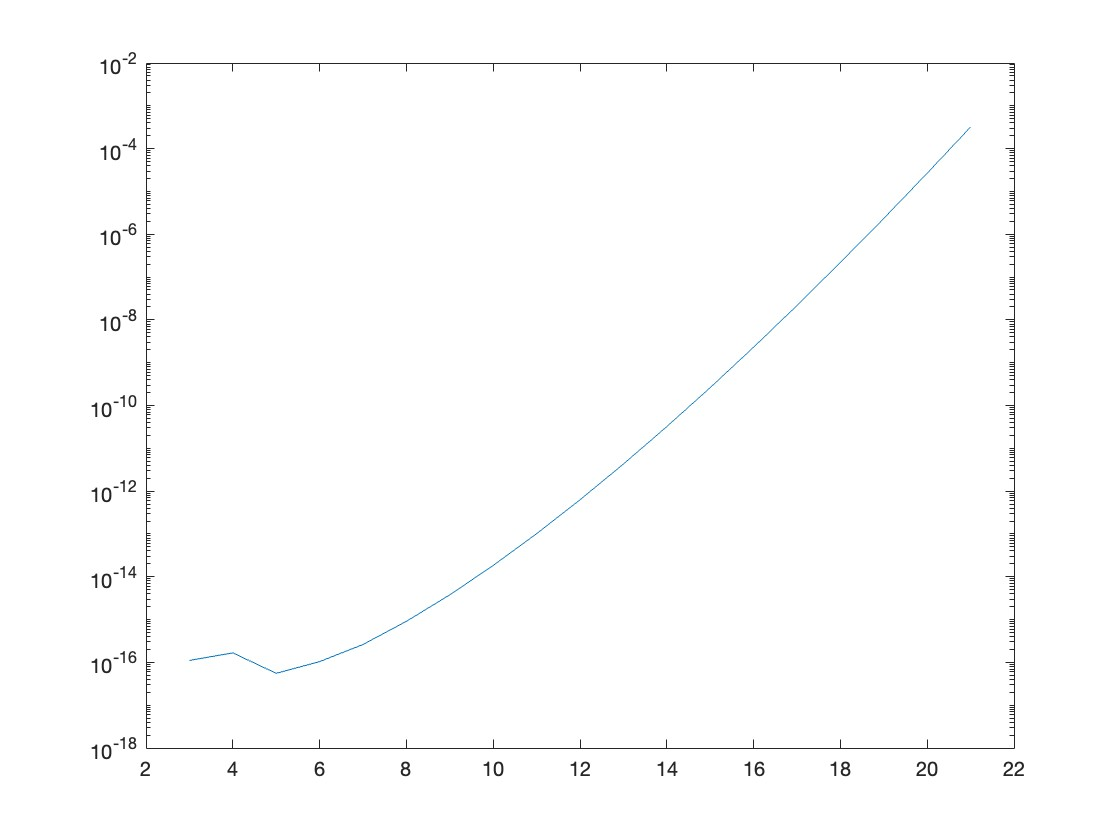
\includegraphics[width=0.7\textwidth]{Hw1-Fig1.jpg}
\end{center}

(ii) Since we know a total sum, and the
recurrence relation is linear, we can be off by
a constant proportion, and correct for it at the
very end. Therefore we can do the recurrence
backwards, ending with \(\dots,c,0\), where \(c\)
is an arbitrary constant. This results in very
large numbers near the beginning, so to compute
more terms, some other measure should be used to
prevent overflowing.
\begin{matlab}
Jpi = [zeros(1,NUM_MAX), 1, 0];
for n = NUM_MAX:-1:1
    Jpi(n) = 2*n*Jpi(n+1) / pi - Jpi(n+2);
end
Jpi = Jpi / (Jpi(1) + 2*sum(Jpi(3:2:NUM_MAX+1)));
Jpi = Jpi(1:NUM_MAX+1);  % Trim off last term

figure(2);
plot(Jpi_accurate - Jpi);
\end{matlab}
\begin{center}
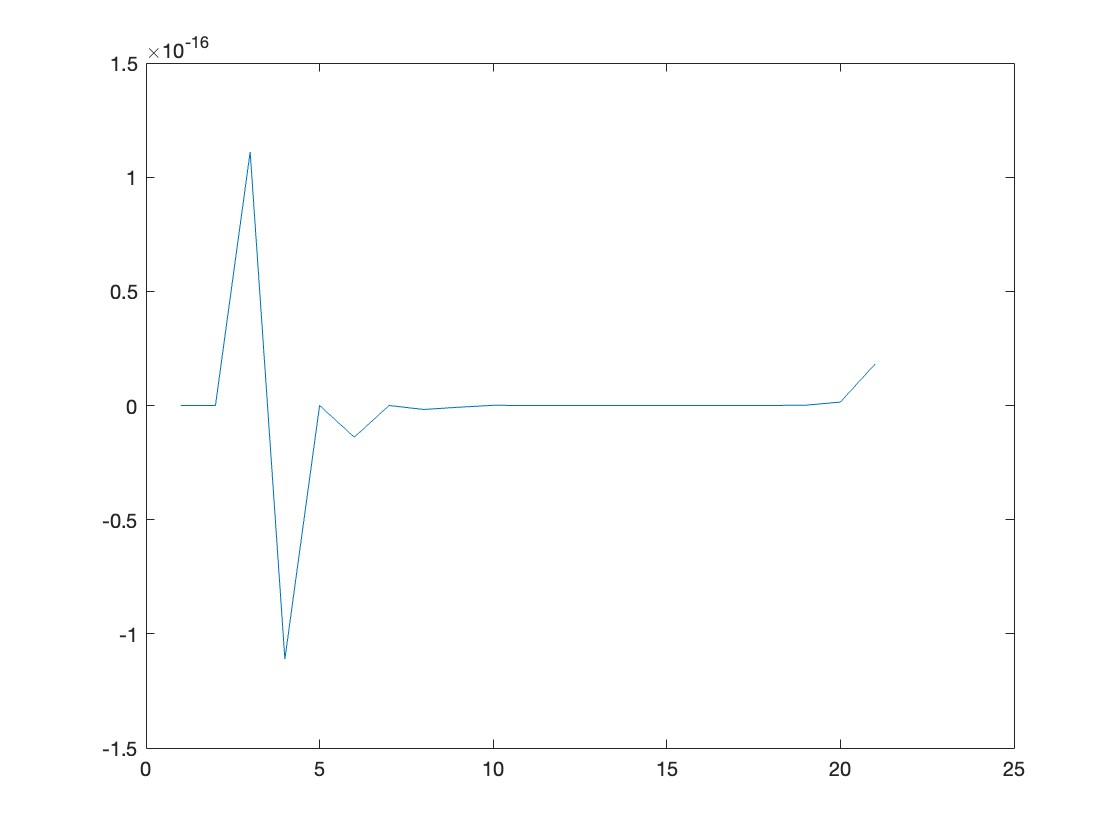
\includegraphics[width=0.7\textwidth]{Hw1-Fig2.jpg}
\end{center}
The result is much more accurate, the error
being around \(10^{-16}\), which is essentially
maximal precision.
\end{problem}

\begin{problem}
The accurate value is expressed by the \(\operatorname{erf}\)
function
\[\int_{-t}^t e^{-x^2}\,\mathrm dx
= \operatorname{erf}(x).\]
\begin{matlab}
I1_accurate = sqrt(pi);
I2_accurate = sqrt(pi) * erf(2);
\end{matlab}
We define the integration function using the
trapezoidal rule:
\begin{matlab}
function int = trapz(fun, left, right, N)
    h = (right-left) / N;
    pts = h * (0:N) + left;
    fpts = fun(pts);
    int = h/2 * sum(fpts(1:N) + fpts(2:N+1));
end
\end{matlab}
Since this method only computes integrals on an
interval, we need to cut off the infinite
integral at some point. Here we choose to cut
it off at \(\pm\sqrt N\). To see how the cut-off
affects the accuracy, we also compute the accurate
values for these integrals.
\begin{matlab}
Ns = (2:50); fun = @(x) exp(-x.^2);

I1_values = arrayfun(@(N) trapz(fun, -sqrt(N), sqrt(N), N), Ns);
I2_values = arrayfun(@(N) trapz(fun, -2, 2, N), Ns);

I1_errors = abs(I1_values - I1_accurate);
I2_errors = abs(I2_values - I2_accurate);
I1_cutoff = sqrt(pi) * (1 - erf(sqrt(Ns)));
\end{matlab}
\begin{center}
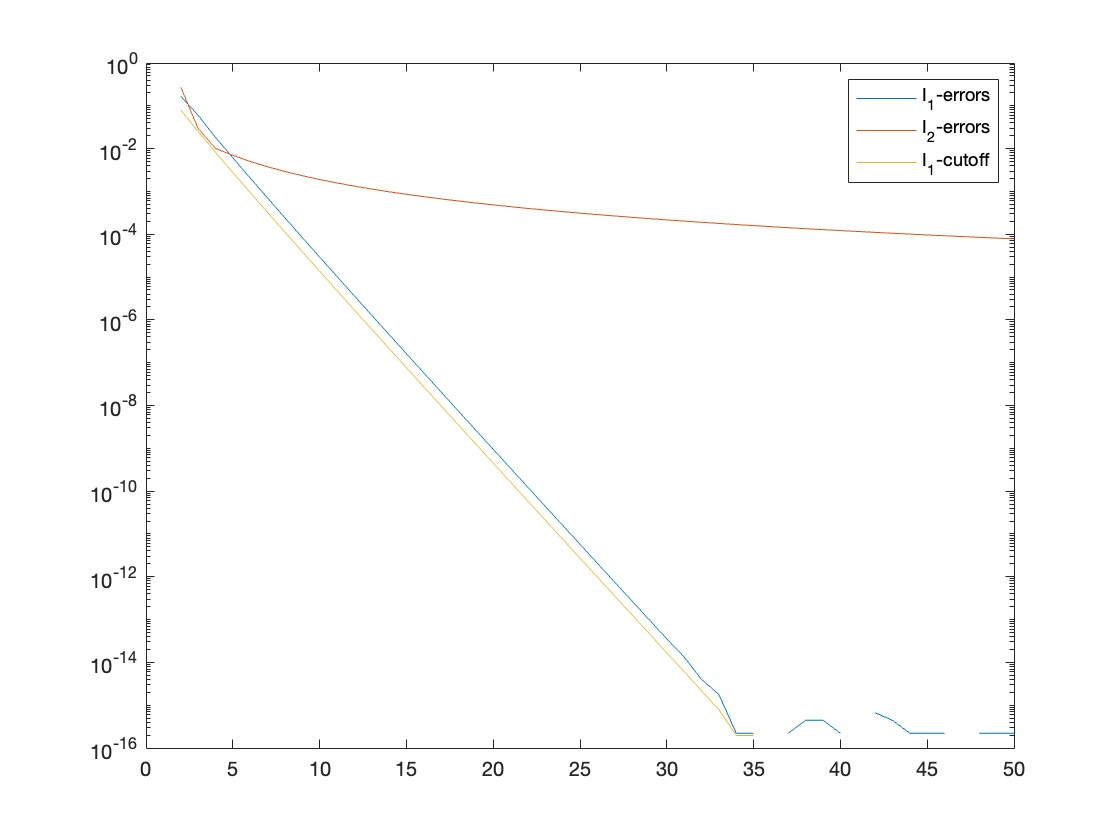
\includegraphics[width=0.8\textwidth]{Hw1-Fig3.jpg}
\end{center}

First we analyze the cut-off error.
Since we have the asymptotics
\[\int_{t}^\infty e^{-x^2} =
\frac{e^{-t^2}}{t\sqrt\pi}
\left[1 + O(t^{-2})\right],\]
the error decreases as \(O(e^{-N}/\sqrt N)\),
and since \(\sqrt N\) is very small compared to
the exponential, the curve on the graph is
almost straight.

However, it is rather surprising that the
integral without the cut-off performs way worse
numerically. To explain this, we need to analyze
the error asymptotics of the trapezoidal rule.
For the interval \([-\frac12,\frac12]\),
integrating by parts twice, we have
\[\begin{aligned}
\int_{-\frac12}^{\frac12} f(x) \d x
&= \frac{f(\frac12) + f(-\frac12)}{2}
 - \int_{-\frac12}^{\frac12} xf'(x)\d x\\
&= \frac{f(\frac12) + f(-\frac12)}{2}
 - \frac12\int_{-\frac12}^{\frac12} x^2\frac{f'(x) - f'(-x)}x\d x\\
&= \frac{f(\frac12) + f(-\frac12)}{2}
 - \frac{f'(\frac12)-f'(-\frac12)}{24}
 + \frac13 \int_{-\frac12}^{\frac12} x^2f''(x) \d x.
\end{aligned}\]
Therefore
\[\int_{-\frac12}^{\frac12} f(x) \d x
= \frac{f(\frac12) + f(-\frac12)}{2}
- \frac{f'(\frac12)-f'(-\frac12)}{24}
+ r.\]
And suppose \(|f''(x)|\) is bounded by \(M\), then
the error term \(|r| \le \frac{M}{12}\). We now
break an integral on \([a,b]\) into \(N\) equal
parts, with endpoints \(a_k = a + k\frac{b-a}{N}\).
Applying this equation on each part:
\[\begin{aligned}
\int_a^b f(x) \d x
&= \sum_{k = 1}^N \int_{a_{k-1}}^{a_k} f(x) \d x\\
&= \sum_{k = 1}^N
\frac{b-a}{N}\underbrace{\frac{f(a_{k-1}) + f(a_k)}{2}}_{\text{trapezoidal}}
+ \left(\frac{b-a}{N}\right)^2\underbrace{\frac{f'(a_{k-1}) - f'(a_k)}{24}}_{\text{telescopic}}
+ \left(\frac{b-a}{N}\right)^3 r_k\\
&= (\text{Trapezoidal}) + \left(\frac{b-a}{N}\right)^2
\left[\frac{f'(a) - f'(b)}{24}\right] + R.
\end{aligned}\]
Letting \(h = \frac{b-a}{N}\), we established
that the trapezoidal rule has error term
\(h^2[f'(a) - f'(b)]/24 + O(h^3)\). Returning
to the original problem, we see that for the
integration on \([-2,2]\), the error term goes
to zero as \(O(N^{-2})\). This roughly agrees
with the data. However for the improper
integral, we took the cut-off at \([-\sqrt N, \sqrt N]\),
so \(|f'(a) - f'(b)| = 4\sqrt Ne^{-N}\) decreases
exponentially as \(N\) increases, and this effect
dwarfs the other factors.

A more rudimentary explication of this phenomenon
is that on concave parts, the trapezoid tends
to underestimate, and on convex parts the reverse.
This error term tends to cancel for \(e^{-x^2}\),
which is concave on some parts, and convex on the
other parts.
\end{problem}

\begin{problem}
(i) For a suitably integrable function
\(f : \mathbb R^2 \to \mathbb R\), we can first
perform a Fourier transform, and then take a
\(y\)-slice, obtaining \(g_1(k) = \hat f(k, 0)\).
We can also first project the function onto
the \(x\)-axis, getting
\(F(x) = \int_{-\infty}^\infty f(x,y)\d y\),
and then performing a Fourier transform, obtaining
\(g_2(k) = \hat F(k)\). The Fourier slice theorem
states that \(g_1 = g_2\).

\begin{proof}
Compute
\[\begin{aligned}
g_1(k)
&= \frac1{\sqrt{2\pi}} \int_{-\infty}^\infty
\int_{-\infty}^\infty e^{ikx + iy\cdot 0} f(x,y) \d x \d y\\
&= \frac1{\sqrt{2\pi}} \int_{-\infty}^\infty
e^{ikx} \int_{-\infty}^\infty f(x,y) \d y \d x\\
&= \frac1{\sqrt{2\pi}} \int_{-\infty}^\infty
e^{ikx} F(x) \d x\\
&= \hat F(k) = g_2(k),
\end{aligned}\]
which concludes the proof, where the integrability
condition is used to invoke Fubini's theorem,
interchanging the integrals.
\renewcommand{\qedsymbol}{\(\square\)}
\end{proof}
\renewcommand{\qedsymbol}{}
\end{problem}

\newpage
\section*{Appendix: Source Code}
\matlabfile{Hw1.m}
\end{document}
